%!TeX encoding=utf8
\documentclass[ngerman]{scrartcl} 

% Passen Sie hier *Author1*, *Author2* und *Grp.-Nr.* an.
\newcommand{\authA}{Alexander Steding}

\newcommand{\grpnr}{4}
\usepackage{array}
\usepackage{longtable}

% Optionen für die Dokumentenklasse scartcl von KOMAscript. 
\KOMAoptions{
	DIV=11,
	BCOR=0mm,
	paper=a4,
	fontsize=12pt,
	parskip=half,
	twoside=false,
	titlepage=false
}
\usepackage{booktabs}

% Papierformat: DIN-A4, mit wenig Rand 
\usepackage[
	a4paper,
	left=20mm,
	right=20mm,
	top=23mm, 
	bottom=18mm,
	includefoot,
	footskip=8mm
	]{geometry}

% Zeilenabstand, andere Werte: onehalfspacing, doublespacing
\usepackage[singlespacing]{setspace} 

% Definition der Kopf- und Fußzeile
\usepackage[headsepline,automark]{scrlayer-scrpage}
\clearscrheadings
\setlength{\headheight}{2.5\baselineskip}
\setlength{\footheight}{1\baselineskip}
\chead[]{ \\  Abschlussbericht}
\ihead[]{\\ \authA}
\ohead[]{Datum: \today }
\ofoot[]{\pagemark}

%---Language and umlauts
\usepackage[utf8]{inputenc}       % UTF-8 Kodierung - ä, ö, ü, ß direkt eingeben
\usepackage[ngerman]{babel}                      % Neue deutsche Rechtschreibung  
\usepackage[expansion=true, protrusion=true]{microtype} % Bessere Silbentrennung

% Formelsatz
\usepackage{amsmath}		% Mathematik-Umgebungen - z.B. align
\usepackage{amsthm}		% Umgebung "theorem"
\usepackage{amsfonts}	% Schriften
\usepackage{amssymb}		% Symbole
\usepackage{upgreek}		% Griechische Sonderzeichen z.B. \upmu
\usepackage{booktabs}
% Einheiten
\usepackage{siunitx}
\sisetup{
	locale = DE,  
	separate-uncertainty,  
	range-units = brackets,  
	list-units = single,  
	per-mode=fraction
}

% Bilder und Tabellen
\usepackage{graphicx}			% Bilder als PDF einbinden
\usepackage{epstopdf}			% Bilder im EPS-Format
\usepackage{caption}				% Unterschriften für Bilder und Tapellen
\usepackage{booktabs}			% Zusätzliche Schönheitslinien für Tabellen
\usepackage{multirow}			% Mehrere Felder in einer Tabelle zusammenfassen
\usepackage[table]{xcolor}		% Für farbig unterlegte Tabellenzeilen
  \definecolor{lightgray}{gray}{0.9}
  \rowcolors{1}{}{lightgray}	% jede zweite Zeile in einer Tabelle leicht grau


% Positionierung von Bildern und Tabellen
\usepackage{float}				% Option 'H', also "hier-egal-wie-das-aussieht"
\usepackage[section]{placeins}	% Platzierung spätestens am Ende eines Kapitels
\renewcommand{\floatpagefraction}{.75}	% standard: .5
\renewcommand{\textfraction}{.1}			% standard: .2
\renewcommand{\topfraction}{.8}			% standard: .7
\renewcommand{\bottomfraction}{.5}		% standard: .3
\setcounter{topnumber}{3}				% standard: 2
\setcounter{bottomnumber}{2}				% standard: 1
\setcounter{totalnumber}{5}				% standard: 3

\usepackage{caption}
\captionsetup[figure]{name=Abb.}
\captionsetup[table]{name=Tab.}

% Hyperlinks
\usepackage{hyperref}
\hypersetup{
	colorlinks=true, 
	breaklinks=true, 
	citecolor=darkgray, 
	linkcolor=darkgray, 
	menucolor=red, 
	urlcolor=cyan,
	bookmarksopen=false, 
	bookmarksopenlevel=0,
	plainpages=false,			% zur korrekten Erstellung der Bookmarks 
	hypertexnames=false			% zur korrekten Erstellung der Bookmarks 
}

\usepackage{pdfpages} 		% Einfügen von Vollseiten-PDFs (z.B. das Deckblatt)
\usepackage{csquotes}		% Zitate
\usepackage{pythonhighlight}
% Literaturverzeichnis
\usepackage[style=alphabetic,sorting=ynt,backend=biber]{biblatex}

% Eine Abkürzung, die Computerbefehle im Fließtext mit einer Mono-Schrift setzt
% (funktioniert leider nicht für Backslash \ . Da hilft dann der Befehl \verb )
\providecommand*{\code}[1]{{\texttt{#1}}}
\usepackage{listings}
\usepackage{xcolor}

\definecolor{codegreen}{rgb}{0,0.6,0}
\definecolor{codegray}{rgb}{0.5,0.5,0.5}
\definecolor{codepurple}{rgb}{0.58,0,0.82}
\definecolor{backcolour}{rgb}{0.95,0.95,0.92}

\lstdefinestyle{mystyle}{
    backgroundcolor=\color{backcolour},   
    commentstyle=\color{codegreen},
    keywordstyle=\color{magenta},
    numberstyle=\tiny\color{codegray},
    stringstyle=\color{codepurple},
    basicstyle=\ttfamily\footnotesize,
    breakatwhitespace=false,         
    breaklines=true,                 
    captionpos=b,                    
    keepspaces=true,                 
    numbers=left,                    
    numbersep=5pt,                  
    showspaces=false,                
    showstringspaces=false,
    showtabs=false,                  
    tabsize=2
}

\lstset{style=mystyle}
\usepackage{hyperref}
\begin{document}
\shorthandoff{"}           % Anführungszeichen nicht als Befehl interpretieren



\begin{titlepage}
\begin{center}
\vspace{3cm}
{\fontsize{40}{49} \selectfont \textbf{Programierpraktikum Übung 4}}\\[2cm]
\Large{\authA }\\
\Large{10028034 }\\
\large{Gottfried Wilhelm Leibniz Universität\\{\today}}
\end{center}
\end{titlepage}
\stepcounter{page}
\tableofcontents  
\newpage

\section{Übung 1}
\section{Ergebnisse}
Gefragt war in dieser Übung nach dem Ort der höchsten Schadstoffkonzentration und nach der Größe dieser. Dazu sollten xy,xz und yz Konturschnitte in jeweils unterschiedlichen Höhen angegeben werden.
\begin{figure}[H]
    \centering
    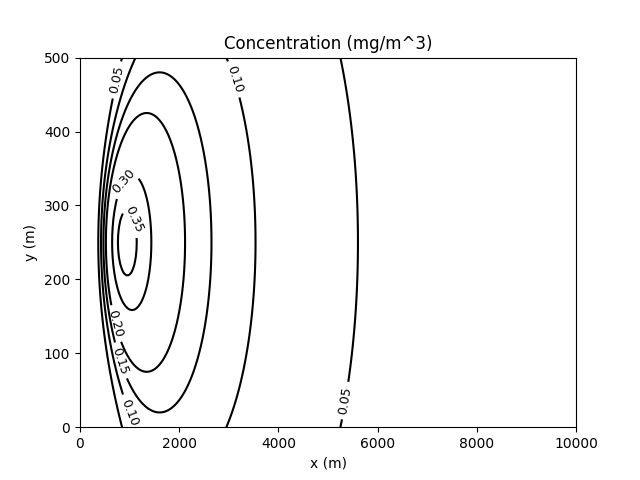
\includegraphics[scale=1]{Übung_1/Bilder/xy_plot.png}
    \caption{Konturschnitt in XY Ebene bei $z=0 \si{m}$}
    \label{fig:my_label}
\end{figure}

\begin{figure}[H]
    \centering
    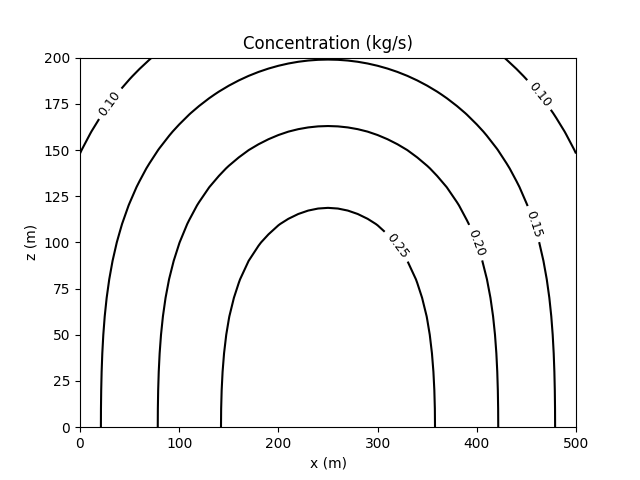
\includegraphics[scale=1]{Übung_1/Bilder/yz_plot.png}
    \caption{Konturschnitt in YZ Ebene bei $x=1000 \si{m}$}
    \label{fig:my_label}
\end{figure}

\begin{figure}[H]
    \centering
    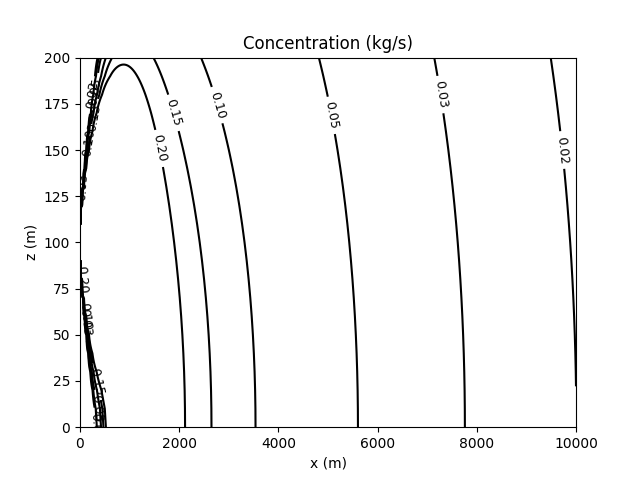
\includegraphics[scale=1]{Übung_1/Bilder/xz_plot.png}
    \caption{Konturschnitt in XZ Ebene bei $y=250 \si{m}$}
    \label{fig:my_label}
\end{figure}
Genauer anaylsiert wurde der Ort der höchsten Konzentration in Fortran selbst. Die größte Konzentration wurde gefunden am Ort:

\begin{equation}
    c(2,26,11)=826,542053 \si{\frac{mg}{m^3}}
\end{equation}
Was dem Ort
\begin{equation}
    r=(10\si{m},250\si{m},100\si{m})
\end{equation}
entspricht.
\section{Übung 2}
\subsection{Partikeltrajektorien}
Gefragt war in dieser Übung nach den Partikeltrajektorien für eine zufällige Linienquelle nach dem Monte Carlo Modell. Für die Berechnung der Partikeltrajektorien und das Visualisieren wurde Python verwendet.
Zunächst mit 10 Partikeln:
\begin{figure}[H]
    \centering
    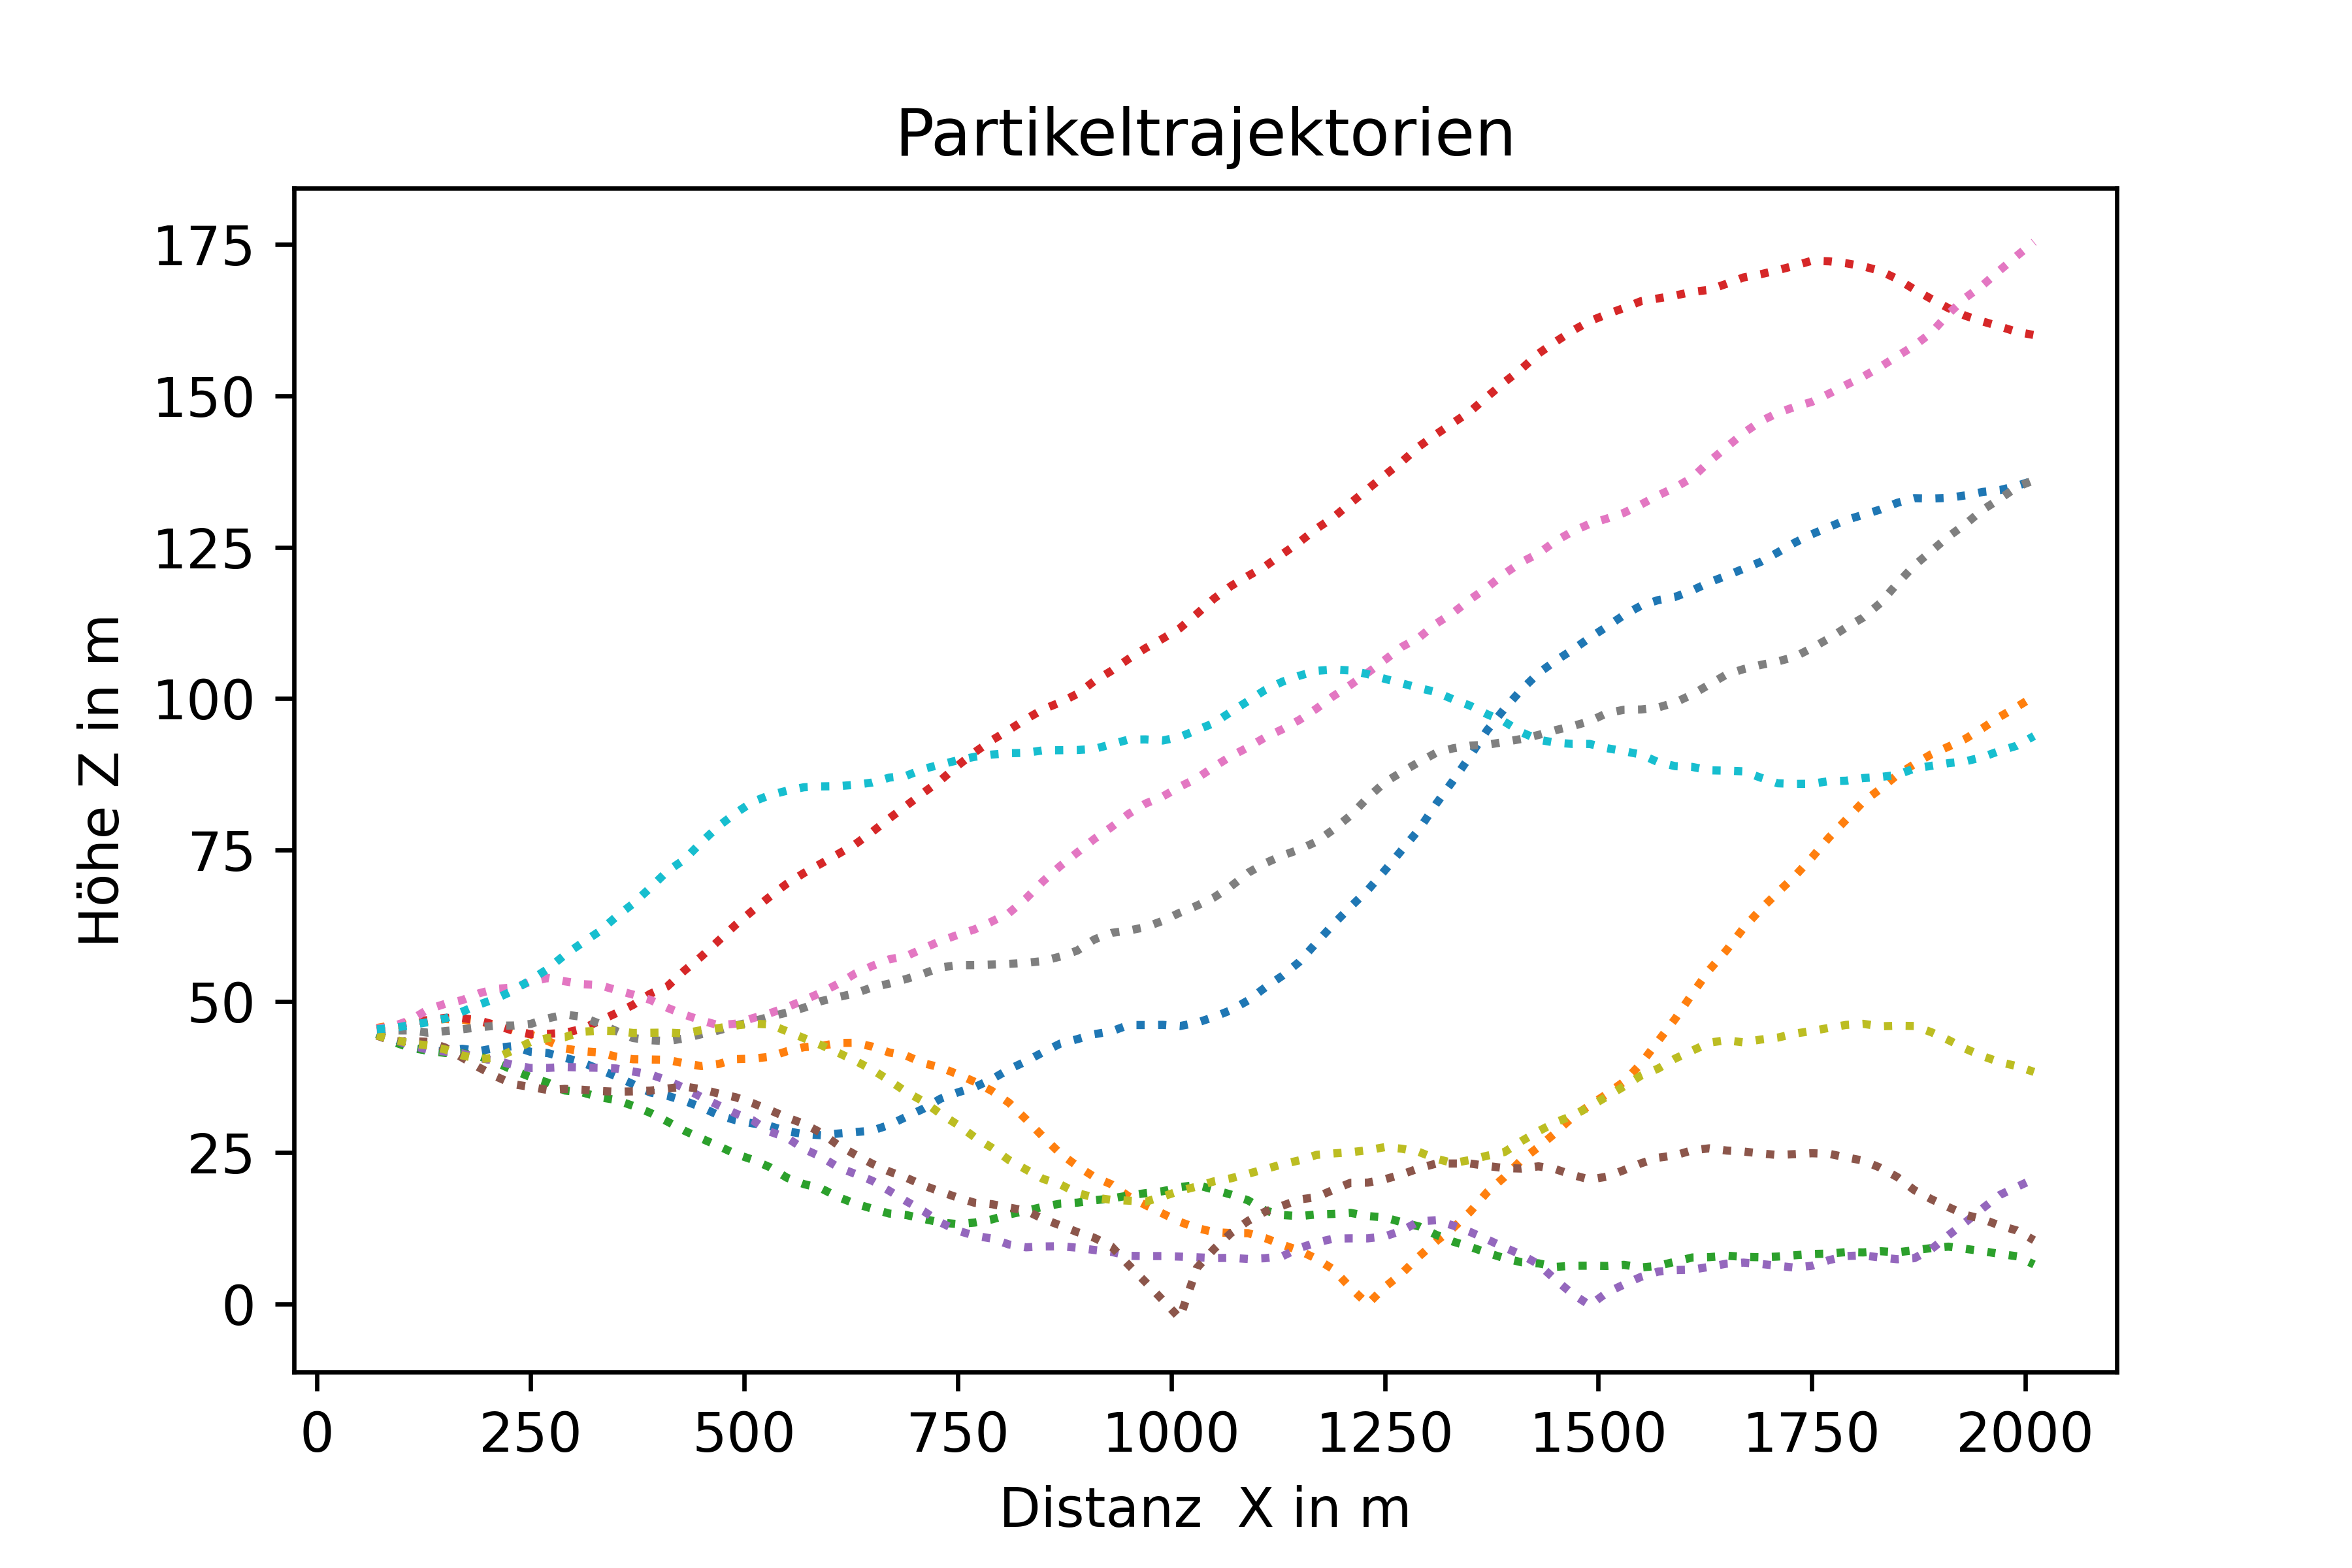
\includegraphics[scale=1]{Übung_2/Bilder/Partikeltrajektorienzehn.png}
    \caption{Trajektorien der einzelnen Parktikel N=10}
    \label{fig:my_label}
\end{figure}
Und Anschließend mit 1000 Partikeln.
\begin{figure}[H]
    \centering
    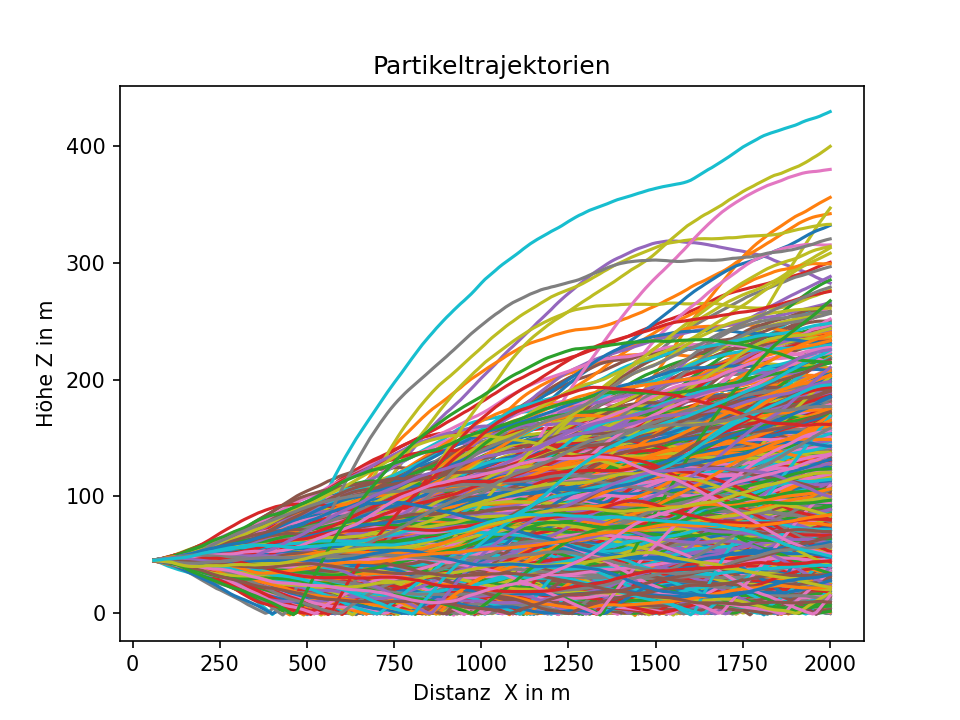
\includegraphics[scale=1]{Übung_2/Bilder/Partikeltrajektorien.png}
    \caption{Trajektorien der einzelnen Parktikel N= 1000}
    \label{fig:my_label}
\end{figure}
\subsection{Vergleich SP und DP}
Im zweiten Aufgabenteil wurde gefragt ob es einen Unterschied macht, ob für die Berechnung der Trajektorien Double oder Single Precission (REAL in Fortran) verwendet wird. Python verwendet standardmäßig Double Precision was einer Bitprezision von 64 bit entspricht. Mithilfe von dem Paket numpy können auch floats mit Single Precision also 32 bit verwendet werden. Um die Unterschiede zu visualisieren wurde jeweils ein  Quotient gebildet:
Zunächst für die X Koordinate:
\begin{figure}[H]
    \centering
    
\includegraphics[scale=1]{Übung_2/Bilder/qX.png}
    \caption{Vergleich DP/SP für die X Koordinate}
    \label{fig:my_label}
\end{figure}
Hier entstehen in der Berechung keine Unterschiede.
Und der Quotient für die Z Koordinate
\begin{figure}[H]
    \centering
    
\includegraphics[scale=1]{Übung_2/Bilder/qZ.png}
    \caption{Vergleich DP/SP für die Z Koordinate}
    \label{fig:my_label}
\end{figure}
Hier entstehen in der Berechnung Unterschiede. Besonders die Berechnungen mit der Zufallszahl weisen leichte Differenzen auf sind aber vernachlässigbar klein bzw nur vereinzelte Partkiel sind betroffen. Im direkten Vergleich


\begin{figure}[H]
    \centering
    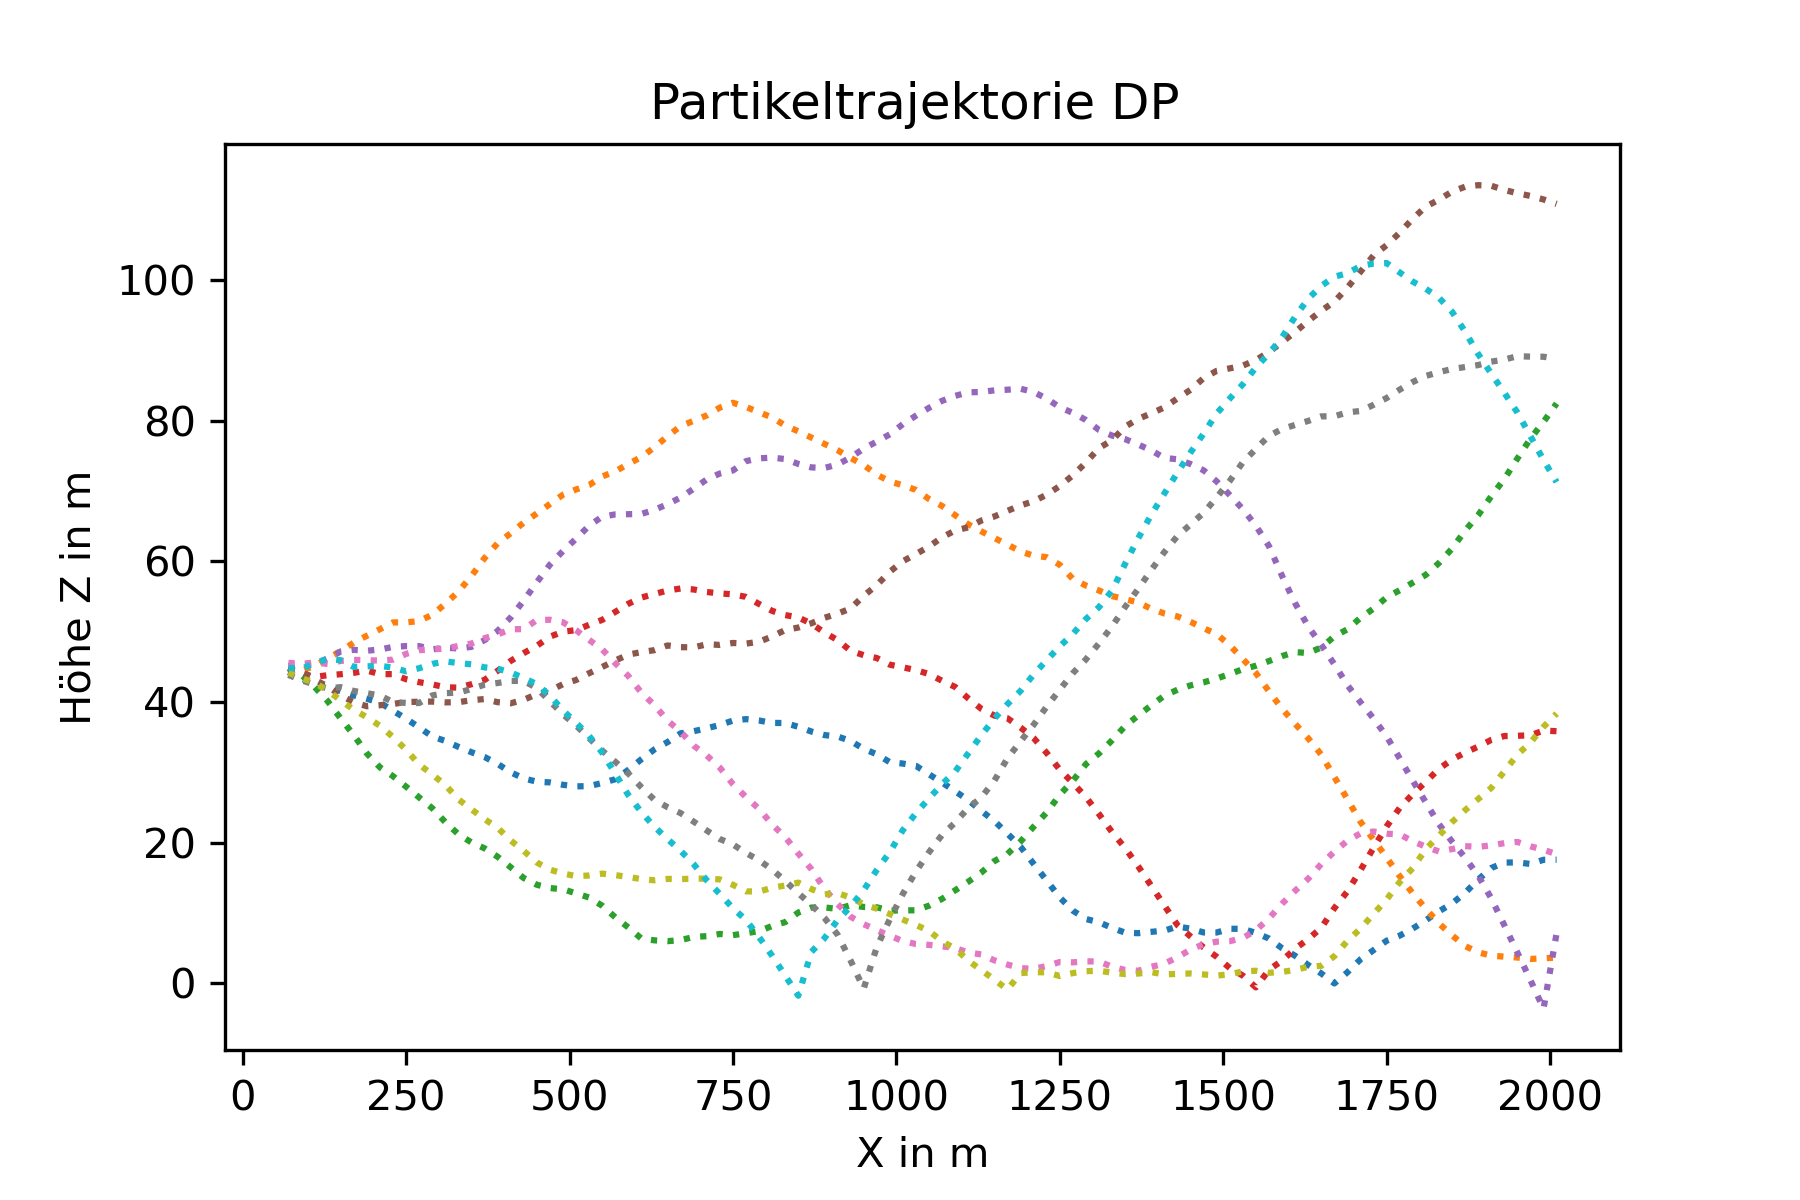
\includegraphics[scale=1]{Übung_2/Bilder/qXh.png}
    \caption{DP Trajektorien}
    \label{fig:my_label}
\end{figure}
\begin{figure}[H]
    \centering
    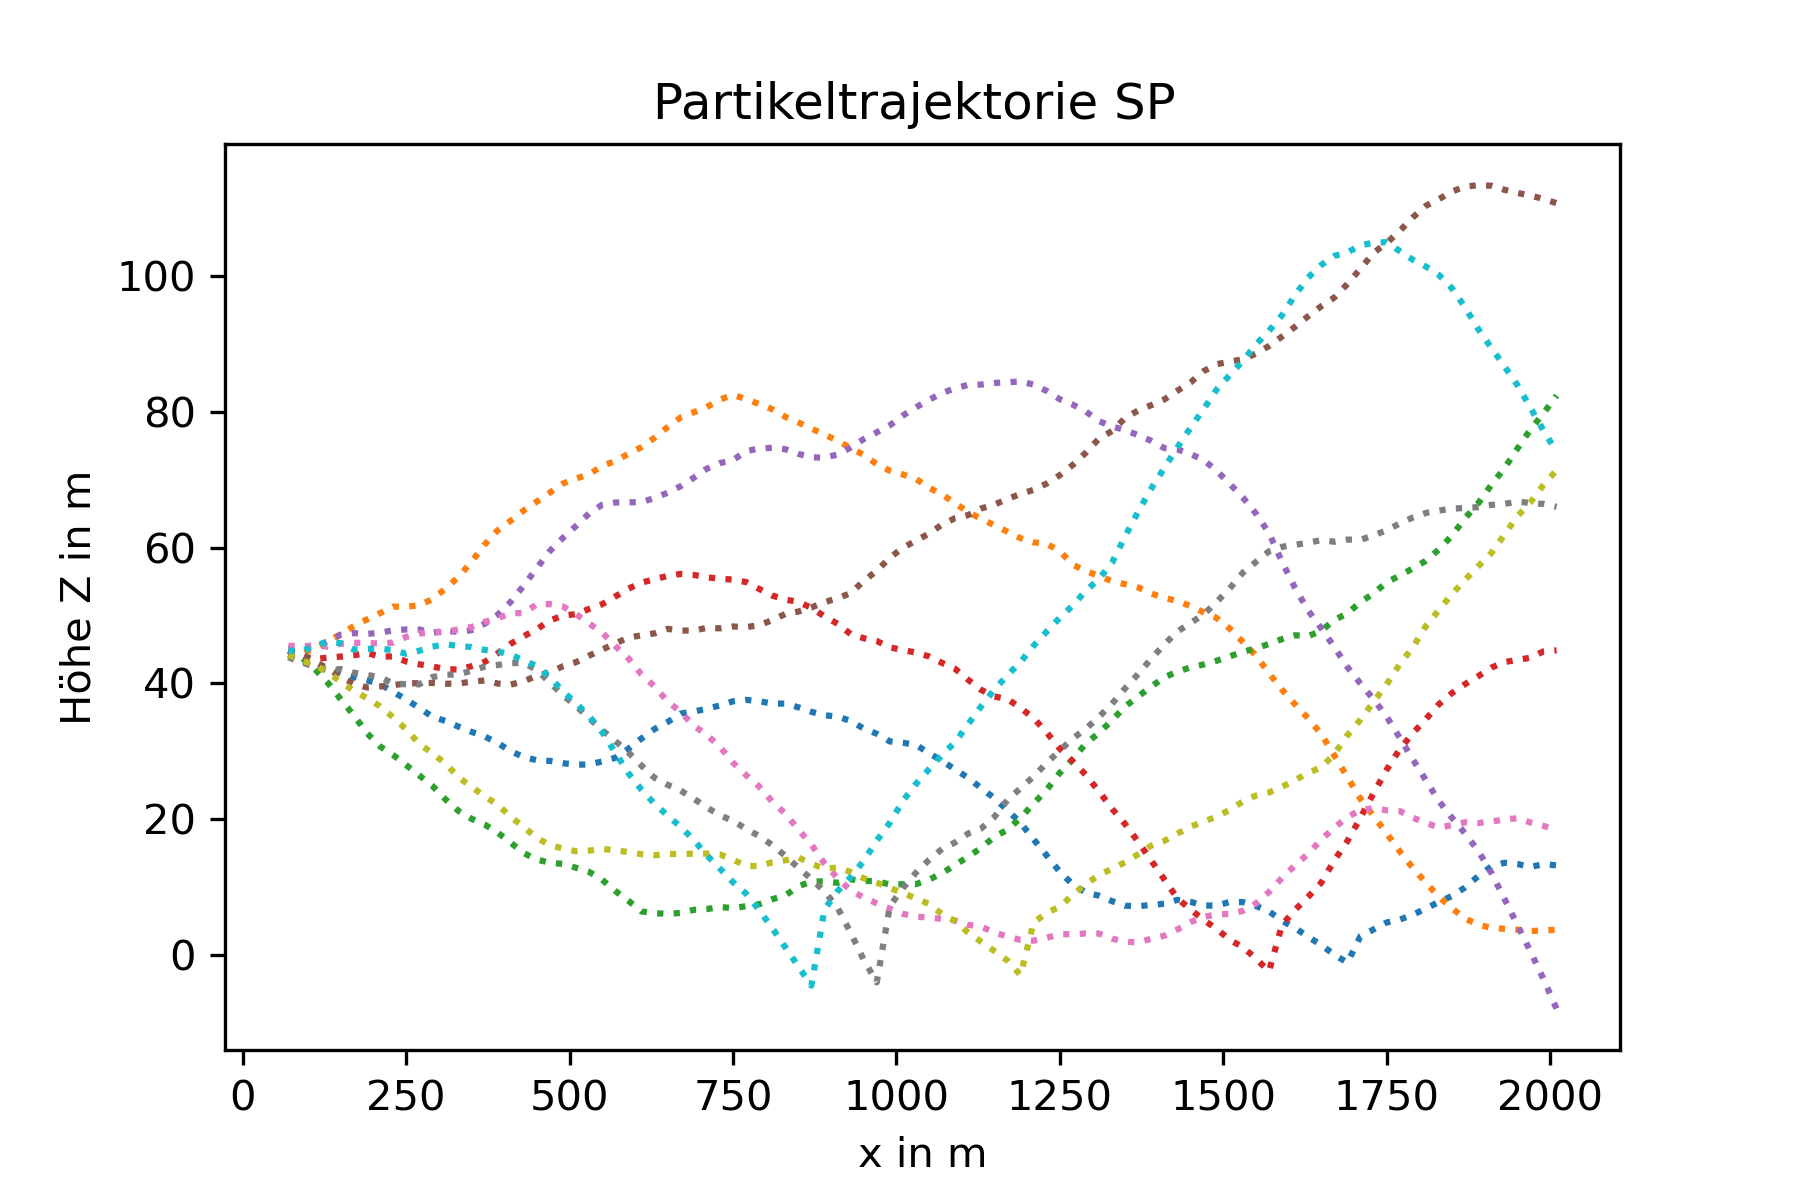
\includegraphics[scale=1]{Übung_2/Bilder/qZh.png}
    \caption{SP Trahjektorien}
    \label{fig:my_label}
\end{figure}

sind diese Unterschiede nicht sichtbar.
\section{Übung 3}

\subsection{Vergleichsplot}
Gefragt war in dieser Übung nach den Unterschieden in der Berechnung  für eine zufällige Linienquelle nach dem Monte Carlo Modell und dem Gaußmodell. Für die Berechnung der Konzentrationen und das Visualisieren wurde Python verwendet.
\begin{figure}[H]
    \centering
    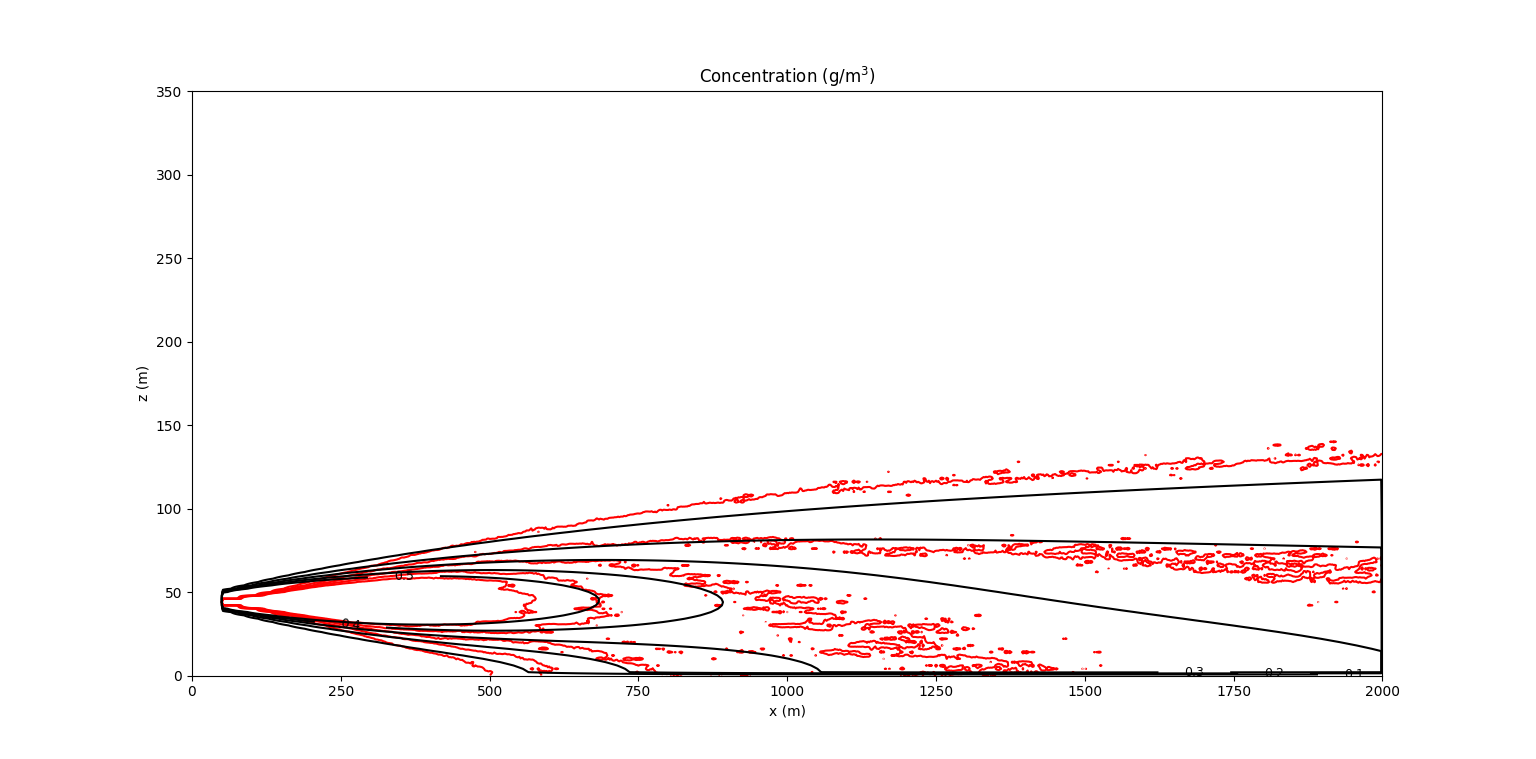
\includegraphics[scale=0.3]{Übung_3/Bilder/30kwide.png}
    \caption{Vergleich MC und Gauß für N=30000}
    \label{fig:my_label}
\end{figure}
In Abb. 1 ist bereits eine gute Annäherung des Montecarlo Modells an das Gaußmodell zu erkennen. Die Anzahl der Teilchen hat beim Montecarlo Modell einen hohen Einfluss auf die Güte des Modells. Bei einer geringeren Anzahl wie 

\begin{equation}
    N=10000
\end{equation}
sind größere Abweichungen zum Gaußmodell zu erkennen.

\begin{figure}[H]
    \centering
    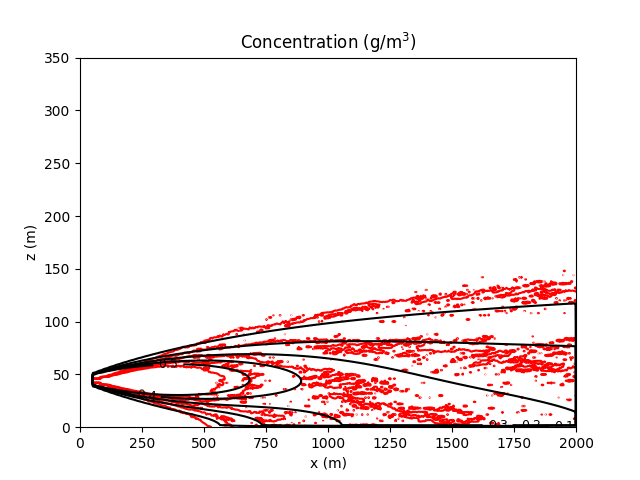
\includegraphics[scale=1]{Übung_3/Bilder/10k.png}
    \caption{Vergleich MC und Gauß für N=10000}
    \label{fig:my_label}
\end{figure}
Bei einer mittleren Anzahl wie 

\begin{equation}
    N=20000
\end{equation}
gleicht sich das MC Modell bedeutend besser an das Gaußmodell an.
\begin{figure}[H]
    \centering
    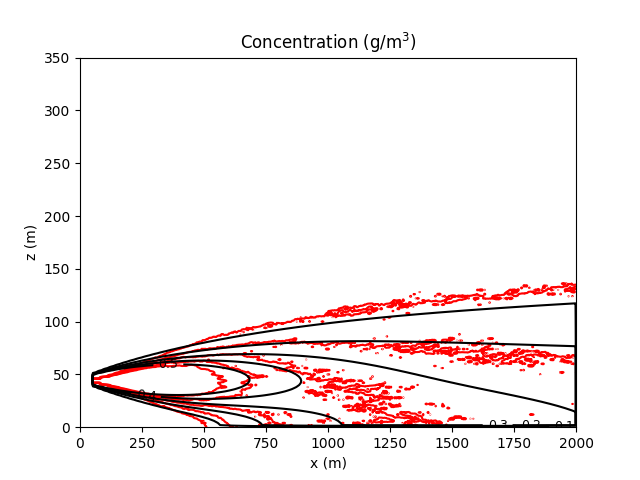
\includegraphics[scale=1]{Übung_3/Bilder/20k.png}
    \caption{Vergleich MC und Gauß für N=20000}
    \label{fig:my_label}
\end{figure}
Bei einer hohen Anzahl wie 

\begin{equation}
    N=30000
\end{equation}
gleicht sich das MC Modell sehr gut an das Gaußmodell an.
\begin{figure}[H]
    \centering
    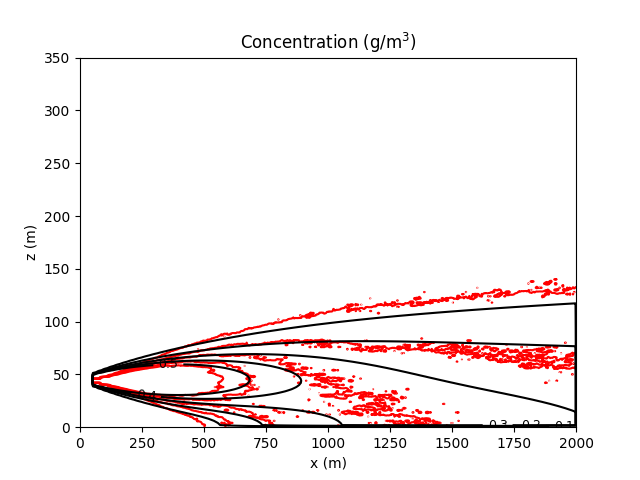
\includegraphics[scale=1]{Übung_3/Bilder/30k.png}
    \caption{Vergleich MC und Gauß für N=30000}
    \label{fig:my_label}
\end{figure}

Trotz Bemühungen Berechnungen innerhalb von Python mittels CUDA auf die GPU auszulagern kam mein Rechner bei höherem N an seine Grenzen. Es bleibt anzunehmen, das ein höheres N nur noch marginale Verbesserung in der Darstellung bewirkt.
\subsection{N und nx}
Im zweiten Aufgabenteil wurde gefragt, wie N nx und nz gewählt werden müssen. Für nx und nz wurde ein Wert von 2000 gewählt, nx und ny spannen so das Gitterrasterauf in denen die Konzentrationen verlaufen sind. Die Anzahl der Partikel bestimmt maßgeblich die Güte des MC Modelle.Bei steigendem N sind können Unterschiede in den Konzentrationen zunehmend feiner aufgelöst werden, auf Kosten der Rechenzeit. in der Übung hat sich ein Wert für n von 30000 als guter Mittelweg erwiesen.Damit muss ich meine vorherige Annahme revidieren.

\section{Übung 4}
\subsection{Vergleichsplot}
Gefragt war in dieser Übung nach einem Vergleich der MonteCarlo Methode und dem Prairie-Grass-Experiment. Zusätlich sollte das MonteCarlo Modell um eine Integration der Prandtlschicht erweitert werden. Eine besondere Herausforderung war zu dem die Integration einer exakten Gitterauswertung. Für die Berechnung der Konzentrationen und das Visualisieren wurde Python verwendet. Dargestellt wurden jeweils die berechnete Konzentrationen mit dem MonteCarlo Modell und die gemessenen Werte aus dem Experiment für verschiedene Höhen.

In dem Praire-Grass-Experiment wurden die Quellstärke nicht weiter konkretisiert, deshalb wurden verschieden Quellstärken ausprobiert. Zunächst mit der Quellstärke

\begin{equation}
Q= 150 \frac{g}{s}
\end{equation}
Dies liefert den folgenden Graphen: 
\begin{figure}[H]
    \centering
    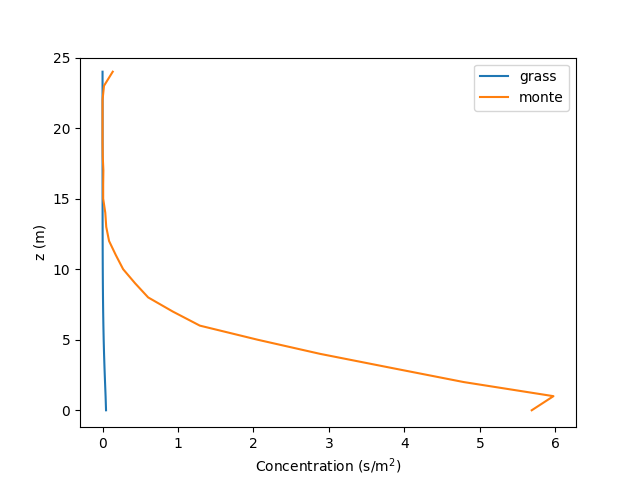
\includegraphics[scale=1]{Übung_4/Bilder/150.png}
    \caption{Vergleich MC und Grass für Q=150}
    \label{fig:my_label}
\end{figure}

Das  MonteCarlo Modell liefert mit diesem Q nur eine sehr schlechte annäherung für Höhen unter 10m.

Ein Q von
\begin{equation}
Q= 0.15 \frac{g}{s}
\end{equation}
 liefert folgenden Graphen:
\begin{figure}[H]
    \centering
    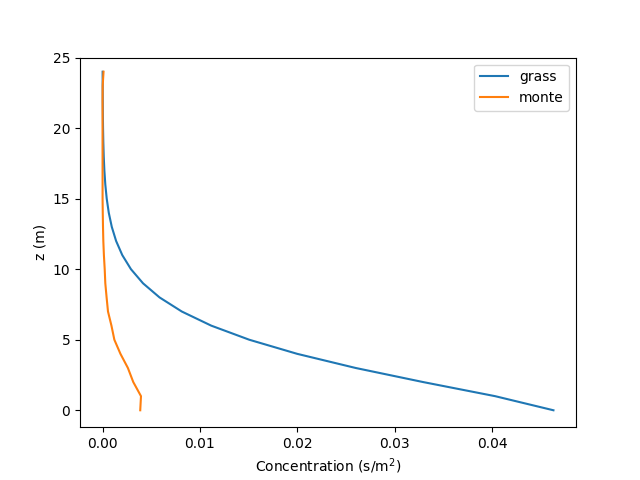
\includegraphics[scale=1]{Übung_4/Bilder/015.png}
    \caption{Vergleich MC und Grass für Q=0.15}
    \label{fig:my_label}
\end{figure}
Diese Quellstärke ist zu gering und das MonteCarlo liefert auch hier nur eine schlechte Anpassung.

Eine Quellstärke von 
\begin{equation}
Q= 1 \frac{g}{s}
\end{equation}
liefert optimale Ergebnisse:
\begin{figure}[H]
    \centering
    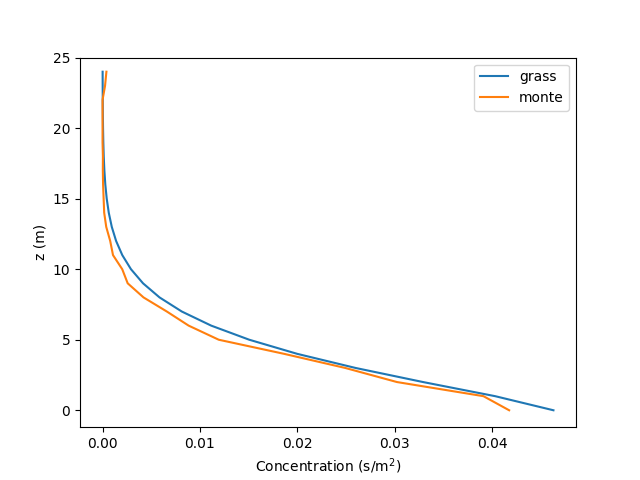
\includegraphics[scale=1]{Übung_4/Bilder/1.png}
    \caption{Vergleich MC und Grass für Q= 1}
    \label{fig:my_label}
\end{figure}

Das MonteCarlo Modell 0schafft hier eine sehr gute Annäherung an das Experiment über alle Höhenbereiche hinweg. Lediglich bei Höhen unter 2m gibt es eine stärkere Abweichung. Dies könnte in der nicht optimierten komplexen Reflexion unter $z_{0}$ liegen, welche in der nächsten Übung in den Ablauf integriert werden kann.


\section{Quellcodes}
\section{Übung2}
\subsection{Python}
\subsubsection{Darstellung}
%\lstinputlisting[language=Python]{Übung_2/Code/bessererdp.py}
\subsubsection{Vergleich DP vs SP}
%\lstinputlisting[language=Python]{Übung_2/Code/vergleich.py}
\subsection{Übung3}
\subsubsection{Darstellung}
%\lstinputlisting[language=Python]{Übung_3/Code/ubung3.py}
\subsubsection{Vergleich Gauss vs MC}
%\lstinputlisting[language=Python]{Übung_3/Code/vergleich_gauss_mc.py}
\subsection{Übung4}
\subsubsection{Angepasstes MC Modell}
%\lstinputlisting[language=Python]{Übung_4/Code/colab.py}
\subsubsection{Darstellung und Vergleich mit dem Grass Experiment}
%\lstinputlisting[language=Python]{Übung_4/Code/grassmodul.py}


\end{document}
